%abstract classes%%%%%%%%%%%%%%%%%%%%%%%%%%%%%%%%%%%%%%%%%%%%%%%%%%%%%%%%%%%%%%%%%%%
% Sensorthing<SensorthingT> 
\rule{\textwidth}{0.4pt}
\class{Sensorthing<SensorthingT>}
\begin{minipage}{0.4\textwidth}
    \begin{figure}[H]
        {\centering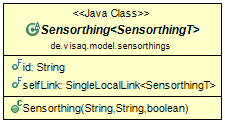
\includegraphics[width=0.95\textwidth]{media/backend/modell/classes/Sensorthing.png}}
    \end{figure}
    \end{minipage} \hfill
    \begin{minipage}{0.6\textwidth}
Die abstrakte Klasse Sensorthing stellt ein Objekt aus der \gls{SensorThings API} da.
Die Klasse vereint die gemeinsamen Eigenschaften der Klassen aus der Datenbank-\gls{API} in sich.
Um die Datentypen der Parameter möglichst exakt zu bestimmen werden \glspl{bounded quantification} verwendet.
\end{minipage}

Attribute:
\begin{itemize}
    \item \emph{public final String id} Jedes Objekt der Datenbank-\gls{API} ist mit einer eindeutigen ID versehen, die das Objekt identifiziert.
    Da sich die ID aus Buchstaben, Zeichen und Ziffern zusammensetzt wird sie hier durch einen String repräsentiert.
    \item \emph{public final SingleLocalLink<SensorthingT> selfLink} Jedes Objekt der \gls{SensorThings API} hält einen Verweis auf die Online-Instanz von sich selbst.
    So kann die Herkunft und die übereinstimmung des Datensatzes mit der Online-Version jederzeit überprüft werden.
\end{itemize}
Methoden: \begin{itemize}
    \item \emph{public Sensorthing(String id, String selfURL, boolean relative)} Diese Methode ist er einzige Konstruktor der Sensorthing-Klasse.
    Als Parameter erhält der Konstruktor neben dem Klassen-Attribut id auch eine URL und eine boolean relative. Beide Parameter werden zum initialisieren des SingleLocalLink benötigt.
\end{itemize}

%%Interfaces%%%%%%%%%%%%%%%%%%%%%%%%%%%%%%%%%%%%%%%%%%%%%%%%%%%%%%%%%%%%%%%%%%%
% SensorthingsProperties
\rule{\textwidth}{0.4pt}
\class{SensorthingsProperties}
\begin{minipage}{0.4\textwidth}
    \begin{figure}[H]
        {\centering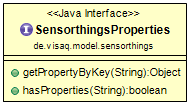
\includegraphics[width=0.95\textwidth]{media/backend/modell/classes/SensorthingsProperties.png}}
    \end{figure}
    \end{minipage} \hfill
\begin{minipage}{0.6\textwidth}
Die Schnittstelle SensorthingsProperties zeigt an, dass ein Objekt der \gls{SensorThings API} Properties besitzt.
Properties sind in diesem Fall Daten vom Typ Object die durch einen String als eindeutigen Identifier gesucht werden können.
Es wird nicht näher spezifiziert welche Properties ein entsprechendes Object muss.
\end{minipage}

Methoden: \begin{itemize}
    \item \emph{public Object getPropertyByKey(String key)} Die Methode sucht in den properties des Objektes eine Eigenschaft mit dem gegebenen Key und gibt den Wert dieser zurück.
    Wenn keine passende Eigenschaft gefunden wurde wird null zurück gegeben.
    \item \emph{public boolean hasProperties(String key)} Die Methode überprüft ob eine Eigenschaft mit dem gegebene Key existiert.
    Falls eine solche Eigenschaft existiert wird true zurück gegeben, andernfalls false.
\end{itemize}

% SensorthingsTimeStamp
\rule{\textwidth}{0.4pt}
\class{SensorthingsTimeStamp}
\begin{minipage}{0.4\textwidth}
    \begin{figure}[H]
        {\centering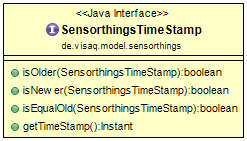
\includegraphics[width=0.95\textwidth]{media/backend/modell/classes/SensorthingsTimeStamp.png}}
    \end{figure}
    \end{minipage} \hfill
\begin{minipage}{0.6\textwidth}
Die Schnittstelle SensorthingsTimeStamp zeigt an, dass ein Objekt der \gls{SensorThings API} einen Zeitstempel besitzt.
Ein Zeitstempel impliziert in diesem Fall, dass zwei solche Objekte anhand ihres Zeitstempels verglichen werden können.
\end{minipage}

Methoden: \begin{itemize}
    \item \emph{public boolean isOlder(SensorthingsTimeStamp other)} Die Methode prüft ob die Instanz älter als die mit other gegebene Instanz ist.
    In diesem Fall wird true zurückgegeben, ansonsten false.
    \item \emph{public boolean isNewer(SensorthingsTimeStamp other)} Die Methode prüft ob die Instanz jünger als die mit other gegebene Instanz ist.
    In diesem Fall wird true zurückgegeben, ansonsten false.
    \item \emph{public boolean isEqualOld(SensorthingsTimeStamp other)} Die Methode prüft ob die Instanz gleich alt wie die mit other gegebene Instanz ist.
    In diesem Fall wird true zurückgegeben, ansonsten false.
    \item \emph{public Instant getTimeStamp()} Die Methode gibt den Zeitstempel als java.time.Instant zurück.
\end{itemize}

%Classes%%%%%%%%%%%%%%%%%%%%%%%%%%%%%%%%%%%%%%%%%%%%%%%%%%%%%%%%%%%%%%%%%%%%%%%
%Datastream
%TODO: Fix class-table size
\rule{\textwidth}{0.4pt}
\class{Datastream extends Sensorthing<Datastream> implements SensorthingsProperties}
\begin{minipage}{0.4\textwidth}
    \begin{figure}[H]
        {\centering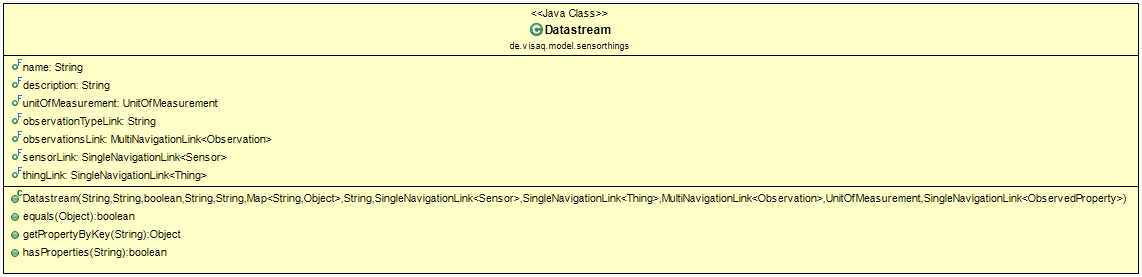
\includegraphics[width=0.95\textwidth]{media/backend/modell/classes/Datastream.png}}
    \end{figure}
    \end{minipage} \hfill
\begin{minipage}{0.6\textwidth}
    \sensorthingsClassDescription{Datastream}{Datastream}
    \url{http://developers.sensorup.com/docs/#datastreams_post}
\end{minipage}

Attribute:
\begin{itemize}
    \item \emph{public final String name} Dieser String repräsentiert den Namen des Datastreams in der Datenbank.
    \item \emph{public final String description} Dieser String stellt repräsentiert die Beschreibung des Datastreams in der Datenbank.
    \item \emph{public final UnitOfMeasurement unitOfMeasurement} Jedem Datastream ist in der Datenbank eine Maßeinheit zugeordnet. Diese maßeinheit wird hier als UnitOfMeasurement gekapselt gespeichert.
    \item \emph{public final String observationTypeLink} Der observationTypeLink gibt an um welchen Typ von Datastream es sich handelt.
    In der Regel wird hier ein Link auf eine Online-Erklärung des Datastream-Typs abgebildet.
    \item \emph{public final MultiNavigationLink<Observation> observationsLink} \multiLinkDescription{Observation}
    \item \emph{public final SingleNavigationLink<Sensor> sensorLink} \singleLinkDescription{Sensor}
    \item \emph{public final SingleNavigationLink<Thing> thingLink} \singleLinkDescription{Thing}
\end{itemize}
Methoden: \begin{itemize}
    \item \emph{public Datastream(String id, String selfUrl, boolean relative, String name, String description, Map<String, Object> properties, String observationTypeLink, SingleNavigationLink<Sensor> sensorLink, SingleNavigationLink<Thing> thingLink, MultiNavigationLink<Observation> observationsLink, UnitOfMeasurement unitOfMeasurement, SingleNavigationLink<ObservedProperty> observedPropertyLink)}
    \constructorDescription{Datastream}
    \item \emph{public boolean equals(Object obj)} \equalsDescriptionWithDB{FeatureOfInterest}
\end{itemize}

%FeatureOfInterest
%TODO: Fix class-table size
\rule{\textwidth}{0.4pt}
\class{FeatureOfInterest extends Sensorthing<FeatureOfInterest>}
\begin{minipage}{0.4\textwidth}
    \begin{figure}[H]
        {\centering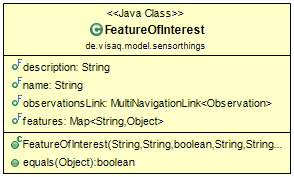
\includegraphics[width=0.95\textwidth]{media/backend/modell/classes/FeatureOfInterest.png}}
    \end{figure}
    \end{minipage} \hfill
\begin{minipage}{0.6\textwidth}
    \sensorthingsClassDescription{FeatureOfInterest}{FeaturesOfInterest}
    \url{http://developers.sensorup.com/docs/#featureOfInterest_post}
\end{minipage}

Attribute:
\begin{itemize}
    \item \emph{public final String name} Dieser String repräsentiert den Namen des FeatureOfInterest in der Datenbank.
    \item \emph{public final String description} Dieser String stellt repräsentiert die Beschreibung des FeatureOfInterest in der Datenbank.
    \item \emph{public final MultiNavigationLink<Observation> observationsLink} \multiLinkDescription{Observation}
    \item \emph{public final Map<String, Object> features} Die in einem FeatureOfInterest gekapselten Informationen werden als Map von String und Object abgelegt.
    Jeder String identifiziert hierbei eindeutig ein Objekt.
\end{itemize}
Methoden:
\begin{itemize}
    \item \emph{public FeatureOfInterest(String id, String selfUrl, boolean relative, String description, String name, MultiNavigationLink<Observation> observationsLink, Map<String, Object> features)}
    \constructorDescription{FeatureOfInterest}
    \item \emph{public boolean equals(Object obj)} \equalsDescriptionWithDB{FeatureOfInterest}
\end{itemize}

%HistoricalLocation
%TODO: Fix class-table size
\rule{\textwidth}{0.4pt}
\class{HistoricalLocation extends Sensorthing<HistoricalLocation>}
\begin{minipage}{0.4\textwidth}
    \begin{figure}[H]
        {\centering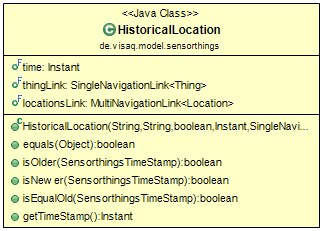
\includegraphics[width=0.95\textwidth]{media/backend/modell/classes/HistoricalLocation.png}}
    \end{figure}
    \end{minipage} \hfill
\begin{minipage}{0.6\textwidth}
    \sensorthingsClassDescription{HistoricalLocation}{HistoricalLocations}
    \url{http://developers.sensorup.com/docs/#historicalLocations_get}
\end{minipage}

Attribute:
\begin{itemize}
    \item \emph{public final Instant time} Der zeitpunkt zudem die Ortsangabe gehört.
    \item \emph{public final SingleNavigationLink<Thing> thingLink} \singleLinkDescription{Thing}
    \item \emph{public final MultiNavigationLink<Location> locationsLink} \multiLinkDescription{Location}
\end{itemize}
Methoden:
\begin{itemize}
    \item \emph{public HistoricalLocation(String id, String selfUrl, boolean relative, Instant time, SingleNavigationLink<Thing> thingLink, MultiNavigationLink<Location> locationsLink)}
    \constructorDescription{HistoricalLocation}
    \item \emph{public boolean equals(Object obj)} \equalsDescriptionWithDB{HistoricalLocation}
\end{itemize}

%Location
%TODO: Fix class-table size
\rule{\textwidth}{0.4pt}
\class{Location extends Sensorthing<Location>}
\begin{minipage}{0.4\textwidth}
    \begin{figure}[H]
        {\centering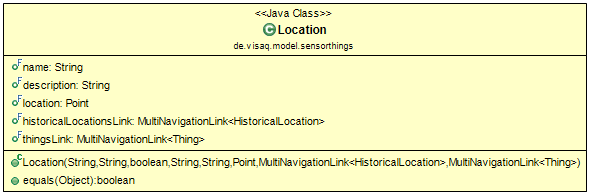
\includegraphics[width=0.95\textwidth]{media/backend/modell/classes/Location.png}}
    \end{figure}
    \end{minipage} \hfill
\begin{minipage}{0.6\textwidth}
    \sensorthingsClassDescription{Location}{Locations}
    \url{http://developers.sensorup.com/docs/#locations_get}
\end{minipage}

Attribute:
\begin{itemize}
    \item \emph{public final String name} Dieser String repräsentiert den Namen der Location in der Datenbank.
    \item \emph{public final String description} Dieser String stellt repräsentiert die Beschreibung der Location in der Datenbank.
    \item \emph{public final Point location} Eine Ortsangabe in Form von Geo-Koordinaten.
    \item \emph{public final MultiNavigationLink<HistoricalLocation> historicalLocationsLink} \multiLinkDescription{HistoricalLocation}
    \item \emph{public final MultiNavigationLink<Thing> thingsLink} \multiLinkDescription{Thing}
\end{itemize}
Methoden:
\begin{itemize}
    \item \emph{public Location(String id, String selfUrl, boolean relative, String name, String description, Point location, MultiNavigationLink<HistoricalLocation> historicalLocationsLink, MultiNavigationLink<Thing> thingsLink)}
    \constructorDescription{Location}
    \item \emph{public boolean equals(Object obj)} \equalsDescriptionWithDB{Location}
\end{itemize}

%Observation
%TODO: Fix class-table size
\rule{\textwidth}{0.4pt}
\class{Observation extends Sensorthing<Observation> implements SensorthingsTimeStamp}
\begin{minipage}{0.4\textwidth}
    \begin{figure}[H]
        {\centering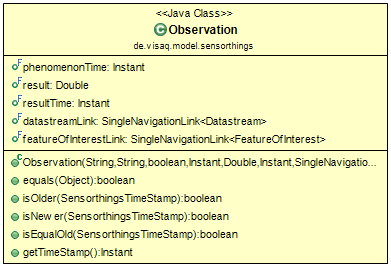
\includegraphics[width=0.95\textwidth]{media/backend/modell/classes/Observation.png}}
    \end{figure}
    \end{minipage} \hfill
\begin{minipage}{0.6\textwidth}
    \sensorthingsClassDescription{Observation}{Observations}
    \url{http://developers.sensorup.com/docs/#observations_post}
\end{minipage}

Attribute:
\begin{itemize}
    \item \emph{public final Instant phenomenonTime} TODO %TODO
    \item \emph{public final Double result} Der Wert den die Beobachtung annimmt
    \item \emph{public final Instant resultTime} TODO %TODO
    \item \emph{public final SingleNavigationLink<Datastream> datastreamLink} \singleLinkDescription{Datastream}
    \item \emph{public final SingleNavigationLink<FeatureOfInterest> featureOfInterestLink} \singleLinkDescription{FeatureOfInterest}
\end{itemize}
Methoden:
\begin{itemize}
    \item \emph{public Observation(String id, String selfUrl, boolean relative, Instant phenomenonTime, Double result, Instant resultTime, SingleNavigationLink<Datastream> datastreamLink, SingleNavigationLink<FeatureOfInterest> featureOfInterestLink)}
    \constructorDescription{Observation}
    \item \emph{public boolean equals(Object obj)} \equalsDescriptionWithDB{Observation}
\end{itemize}

%ObservedProperty
%TODO: Fix class-table size
\rule{\textwidth}{0.4pt}
\class{ObservedProperty extends Sensorthing<ObservedProperty>}
\begin{minipage}{0.4\textwidth}
    \begin{figure}[H]
        {\centering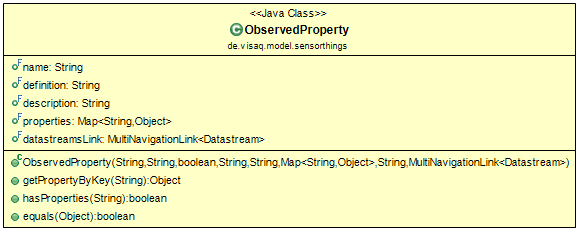
\includegraphics[width=0.95\textwidth]{media/backend/modell/classes/ObservedProperty.png}}
    \end{figure}
    \end{minipage} \hfill
\begin{minipage}{0.6\textwidth}
    \sensorthingsClassDescription{ObservedProperty}{ObservedProperty}
    \url{http://developers.sensorup.com/docs/#observedProperties_post}
\end{minipage}

Attribute:
\begin{itemize}
    \item \emph{public final String name} Dieser String repräsentiert den Namen des ObservedPropertys in der Datenbank.
    \item \emph{public final String description} Dieser String stellt repräsentiert die Beschreibung des ObservedPropertys in der Datenbank.
    \item \emph{public final String definition} Eine formale definition des ObservedPropertys 
    \item \emph{public final Map<String, Object> properties} Die Eigenschaften des ObservedPropertys werden als Map von String und Object gespeichert. Die Strings sind hierbei eindeutig und identifizieren genau ein Objekt der Map.
    \item \emph{public final MultiNavigationLink<Datastream> datastreamsLink} \multiLinkDescription{Datastream}
\end{itemize}
Methoden:
\begin{itemize}
    \item \emph{public ObservedProperty(String id, String selfUrl, boolean relative, String description, String name, Map<String, Object> properties, String definition, MultiNavigationLink<Datastream> datastreamsLink)}
    \constructorDescription{ObservedProperty}
    \item \emph{public boolean equals(Object obj)} \equalsDescriptionWithDB{ObservedProperty}
\end{itemize}

%Sensor
%TODO: Fix class-table size
\rule{\textwidth}{0.4pt}
\class{Sensor extends Sensorthing<Sensor> implements SensorthingsProperties}
\begin{minipage}{0.4\textwidth}
    \begin{figure}[H]
        {\centering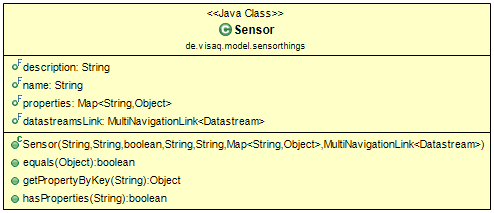
\includegraphics[width=0.95\textwidth]{media/backend/modell/classes/Sensor.png}}
    \end{figure}
    \end{minipage} \hfill
\begin{minipage}{0.6\textwidth}
    \sensorthingsClassDescription{Sensor}{Sensor}
    \url{https://developers.sensorup.com/docs/#sensors_post}
\end{minipage}

Attribute:
\begin{itemize}
    \item \emph{public final String name} Dieser String repräsentiert den Namen des ObservedPropertys in der Datenbank.
    \item \emph{public final String description} Dieser String stellt repräsentiert die Beschreibung des ObservedPropertys in der Datenbank.
    \item \emph{public final Map<String, Object> properties} Die Eigenschaften des Sensors werden als Map von String und Object gespeichert. Die Strings sind hierbei eindeutig und identifizieren genau ein Objekt der Map.
    \item \emph{public final MultiNavigationLink<Datastream> datastreamsLink} \multiLinkDescription{Datastream}
\end{itemize}
Methoden:
\begin{itemize}
    \item \emph{public Sensor(String id, String selfUrl, boolean relative, String description, String name, Map<String, Object> properties, MultiNavigationLink<Datastream> datastreamsLink)}
    \constructorDescription{Sensor}
    \item \emph{public boolean equals(Object obj)} \equalsDescriptionWithDB{Sensor}
\end{itemize}

%Thing
%TODO: Fix class-table size
\rule{\textwidth}{0.4pt}
\class{Thing extends Sensorthing<Thing> implements SensorthingsProperties}
\begin{minipage}{0.4\textwidth}
    \begin{figure}[H]
        {\centering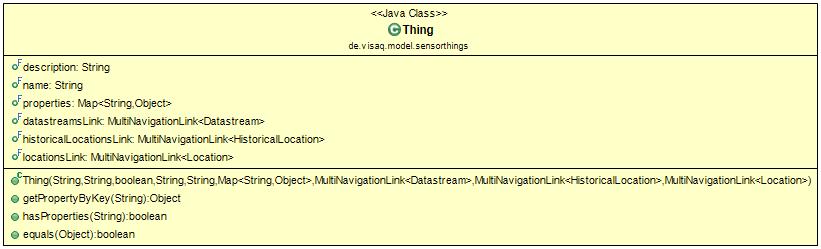
\includegraphics[width=0.95\textwidth]{media/backend/modell/classes/Thing.png}}
    \end{figure}
    \end{minipage} \hfill
\begin{minipage}{0.6\textwidth}
    \sensorthingsClassDescription{Thing}{Things}
    \url{https://developers.sensorup.com/docs/#things}
\end{minipage}

Attribute:
\begin{itemize}
    \item \emph{public final String name} Dieser String repräsentiert den Namen des ObservedPropertys in der Datenbank.
    \item \emph{public final String description} Dieser String stellt repräsentiert die Beschreibung des ObservedPropertys in der Datenbank.
    \item \emph{public final Map<String, Object> properties} Die Eigenschaften des Things werden als Map von String und Object gespeichert. Die Strings sind hierbei eindeutig und identifizieren genau ein Objekt der Map.
    \item \emph{public final MultiNavigationLink<Datastream> datastreamsLink} \multiLinkDescription{Datastream}
    \item \emph{public final MultiNavigationLink<HistoricalLocation> historicalLocationsLink} \multiLinkDescription{HistoricalLocation}
    \item \emph{public final MultiNavigationLink<Location> locationsLink} \multiLinkDescription{Location}
\end{itemize}
Methoden:
\begin{itemize}
    \item \emph{public Thing(String id, String selfUrl, boolean relative, String description, String name, Map<String, Object> properties, MultiNavigationLink<Datastream> datastreamsLink, MultiNavigationLink<HistoricalLocation> historicalLocationsLink, MultiNavigationLink<Location> locationsLink)}
    \constructorDescription{Thing}
    \item \emph{public boolean equals(Object obj)} \equalsDescriptionWithDB{Thing}
\end{itemize}

%UnitOfMeasurement
\rule{\textwidth}{0.4pt}
\class{UnitOfMeasurement}
\begin{minipage}{0.4\textwidth}
    \begin{figure}[H]
        {\centering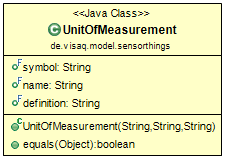
\includegraphics[width=0.95\textwidth]{media/backend/modell/classes/UnitOfMeasurement.png}}
    \end{figure}
    \end{minipage} \hfill
\begin{minipage}{0.6\textwidth}
    Die Klasse UnitOfMeasurement beschreibt eine Maßeinheit für einen Datastream
\end{minipage}

Attribute:
\begin{itemize}
    \item \emph{public final String symbol} Das Symbol der Maßeinheit, wie es zum Beispiel bei der Angabe von Werten mit dieser einheit Benutzt wird.
    \item \emph{public final String name} Der Name der Maßeinheit.
    \item \emph{public final String definition} Eine Definition der Maßeinheit
\end{itemize}
Methoden:
\begin{itemize}
    \item \emph{public UnitOfMeasurement(String name, String symbol, String definition)}
    \constructorDescription{Thing}
    \item \emph{public boolean equals(Object obj)} \equalsDescription{UniteofMeasurement}
\end{itemize}
